\documentclass{standalone}
\usepackage{tikz}
\usetikzlibrary{patterns, positioning}
\usepackage[sfdefault]{ClearSans} %% option 'sfdefault' activates Clear Sans as the default text font
\usepackage[T1]{fontenc}

\begin{document}
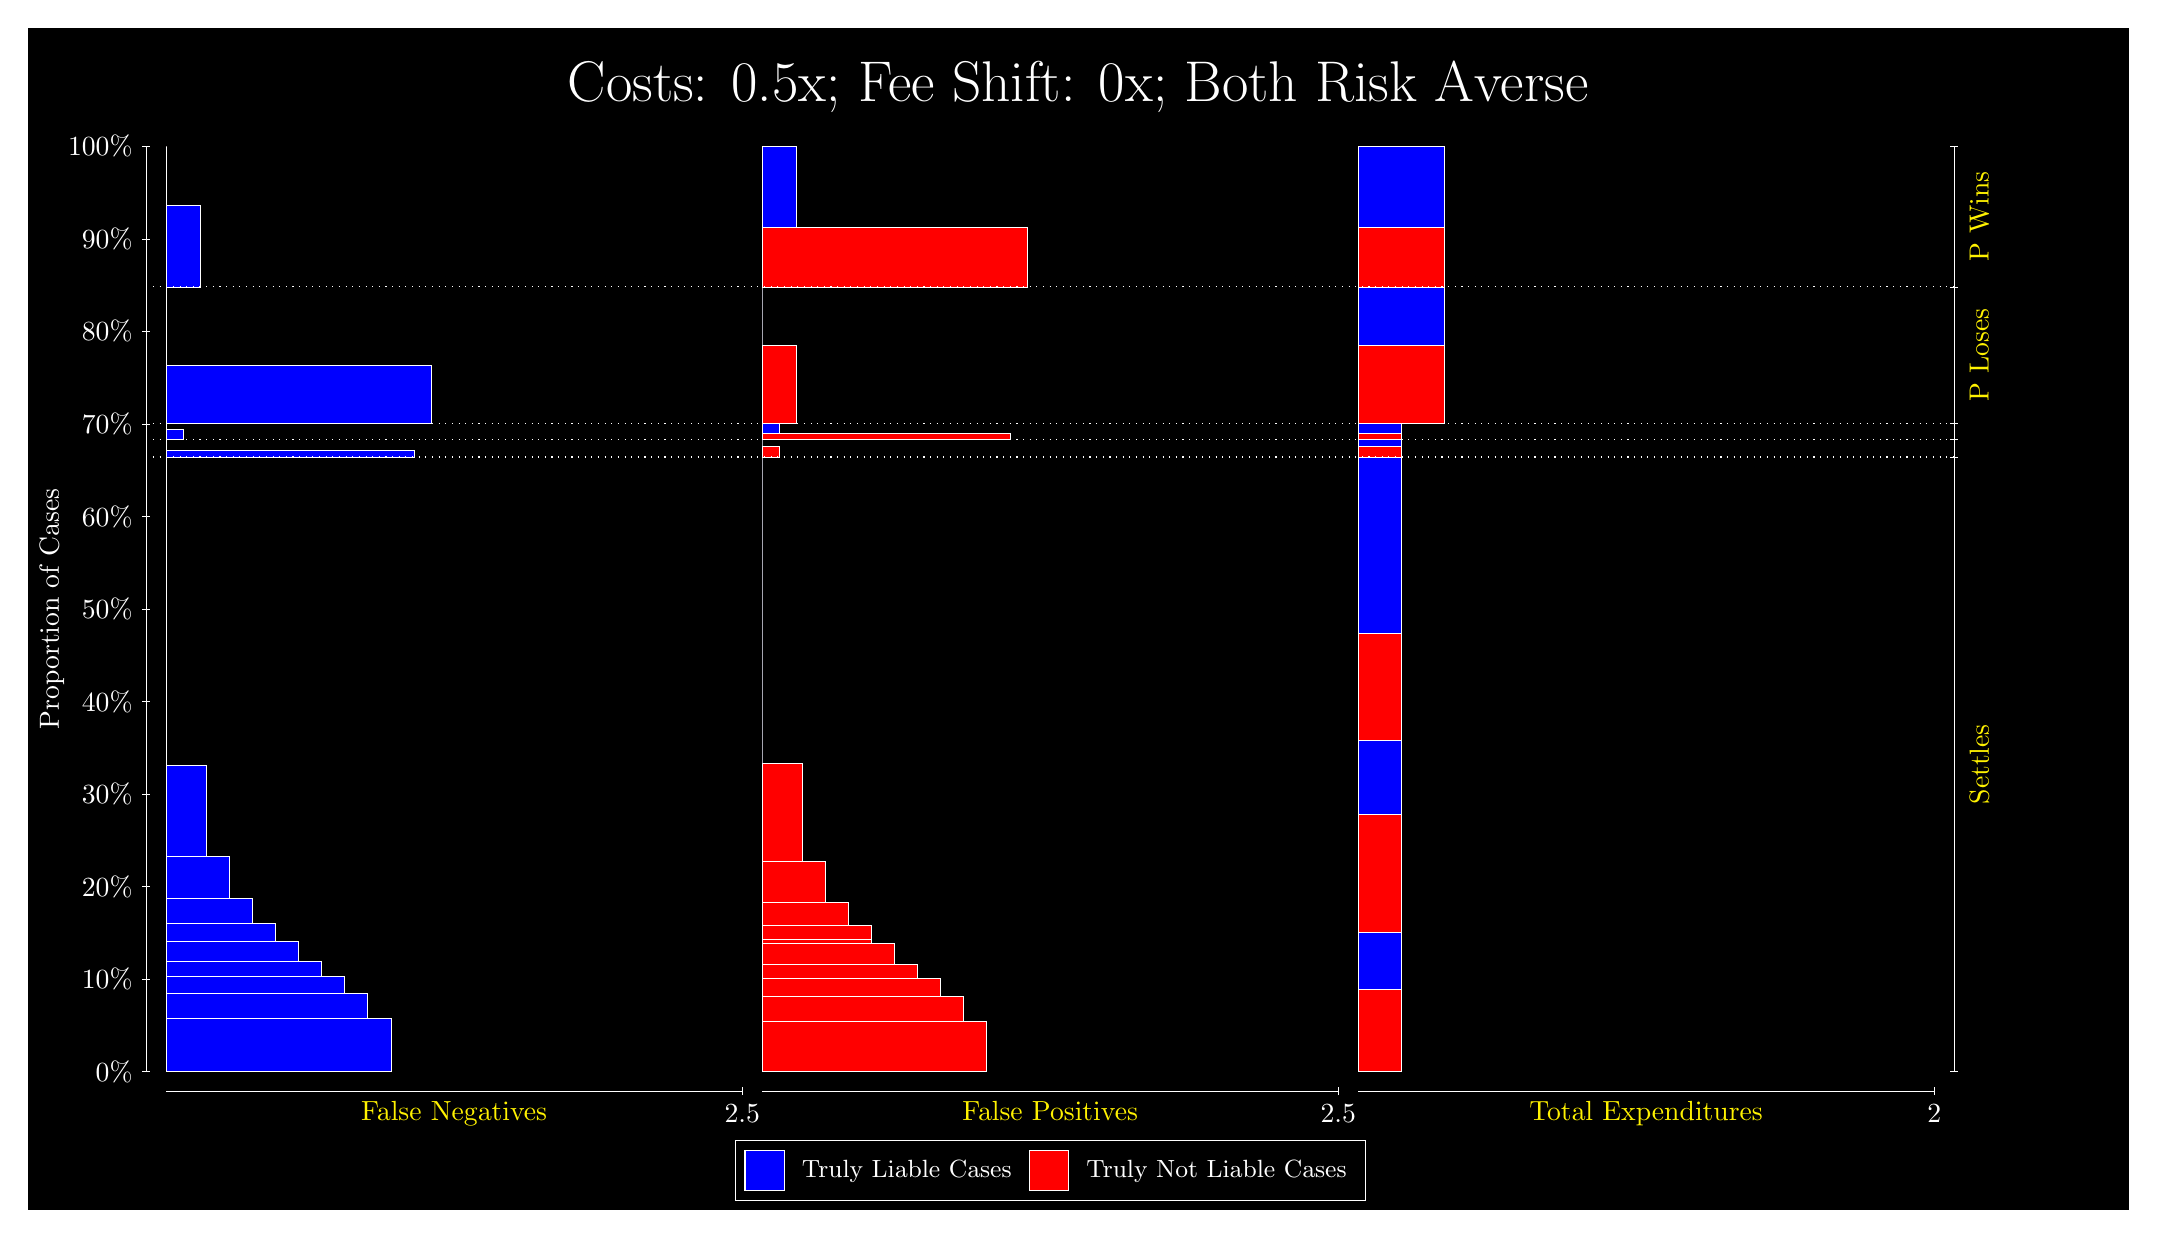
\begin{tikzpicture}
\draw[fill=black] (0,0) rectangle (26.667,15);
\draw[text=white] (0,13.5) rectangle (26.667,15) node[midway] {\huge Costs: 0.5x; Fee Shift: 0x; Both Risk Averse};
\draw[white, very thin] (1.5,1.75) -- (1.5,13.5);
\node[rotate=90, text=white, anchor=center] at (0.3, 7.625) {Proportion of Cases};
\draw[white, very thin] (1.45,1.75) -- (1.55,1.75);
\node[text=white, anchor=east] at (1.45, 1.75) {0\%};
\draw[white, very thin] (1.45,2.925) -- (1.55,2.925);
\node[text=white, anchor=east] at (1.45, 2.925) {10\%};
\draw[white, very thin] (1.45,4.1) -- (1.55,4.1);
\node[text=white, anchor=east] at (1.45, 4.1) {20\%};
\draw[white, very thin] (1.45,5.275) -- (1.55,5.275);
\node[text=white, anchor=east] at (1.45, 5.275) {30\%};
\draw[white, very thin] (1.45,6.45) -- (1.55,6.45);
\node[text=white, anchor=east] at (1.45, 6.45) {40\%};
\draw[white, very thin] (1.45,7.625) -- (1.55,7.625);
\node[text=white, anchor=east] at (1.45, 7.625) {50\%};
\draw[white, very thin] (1.45,8.8) -- (1.55,8.8);
\node[text=white, anchor=east] at (1.45, 8.8) {60\%};
\draw[white, very thin] (1.45,9.975) -- (1.55,9.975);
\node[text=white, anchor=east] at (1.45, 9.975) {70\%};
\draw[white, very thin] (1.45,11.15) -- (1.55,11.15);
\node[text=white, anchor=east] at (1.45, 11.15) {80\%};
\draw[white, very thin] (1.45,12.325) -- (1.55,12.325);
\node[text=white, anchor=east] at (1.45, 12.325) {90\%};
\draw[white, very thin] (1.45,13.5) -- (1.55,13.5);
\node[text=white, anchor=east] at (1.45, 13.5) {100\%};

\draw[white, very thin] (24.457,1.75) -- (24.457,13.5);
\draw[white, very thin] (24.407,1.75) -- (24.507,1.75);
\node[anchor=west] at (24.407, 1.75) {};
\draw[white, very thin] (24.407,9.5541) -- (24.507,9.5541);
\node[anchor=west] at (24.407, 9.5541) {};
\draw[white, very thin] (24.407,9.7757) -- (24.507,9.7757);
\node[anchor=west] at (24.407, 9.7757) {};
\draw[white, very thin] (24.407,9.9797) -- (24.507,9.9797);
\node[anchor=west] at (24.407, 9.9797) {};
\draw[white, very thin] (24.407,11.716) -- (24.507,11.716);
\node[anchor=west] at (24.407, 11.716) {};
\draw[white, very thin] (24.407,13.5) -- (24.507,13.5);
\node[anchor=west] at (24.407, 13.5) {};

\draw[white, very thin, fill=blue] (1.75,1.75) rectangle (4.6044,2.4314);
\draw[white, very thin, fill=blue] (1.75,2.4314) rectangle (4.3116,2.7427);
\draw[white, very thin, fill=blue] (1.75,2.7427) rectangle (4.0188,2.966);
\draw[white, very thin, fill=blue] (1.75,2.966) rectangle (3.7261,3.1511);
\draw[white, very thin, fill=blue] (1.75,3.1511) rectangle (3.4333,3.4098);
\draw[white, very thin, fill=blue] (1.75,3.4098) rectangle (3.1406,3.6351);
\draw[white, very thin, fill=blue] (1.75,3.6351) rectangle (2.8478,3.9504);
\draw[white, very thin, fill=blue] (1.75,3.9504) rectangle (2.5551,4.479);
\draw[white, very thin, fill=blue] (1.75,4.479) rectangle (2.2623,5.6449);
\draw[white, very thin, fill=red] (1.75,5.6449) rectangle (1.75,9.5541);
\draw[white, very thin, fill=blue] (1.75,9.5541) rectangle (4.8971,9.6394);
\draw[white, very thin, fill=red] (1.75,9.6394) rectangle (1.75,9.7757);
\draw[white, very thin, fill=blue] (1.75,9.7757) rectangle (1.9696,9.9011);
\draw[white, very thin, fill=red] (1.75,9.9011) rectangle (1.75,9.9797);
\draw[white, very thin, fill=blue] (1.75,9.9797) rectangle (5.1167,10.718);
\draw[white, very thin, fill=red] (1.75,10.718) rectangle (1.75,11.716);
\draw[white, very thin, fill=blue] (1.75,11.716) rectangle (2.1891,12.747);
\draw[white, very thin, fill=red] (1.75,12.747) rectangle (1.75,13.5);
\draw[white, very thin, fill=red] (9.3189,1.75) rectangle (12.173,2.3888);
\draw[white, very thin, fill=red] (9.3189,2.3888) rectangle (11.88,2.7053);
\draw[white, very thin, fill=red] (9.3189,2.7053) rectangle (11.588,2.9356);
\draw[white, very thin, fill=red] (9.3189,2.9356) rectangle (11.295,3.117);
\draw[white, very thin, fill=red] (9.3189,3.117) rectangle (11.002,3.3741);
\draw[white, very thin, fill=red] (9.3189,3.3741) rectangle (10.709,3.4275);
\draw[white, very thin, fill=red] (9.3189,3.4275) rectangle (10.709,3.6019);
\draw[white, very thin, fill=red] (9.3189,3.6019) rectangle (10.417,3.9019);
\draw[white, very thin, fill=red] (9.3189,3.9019) rectangle (10.124,4.4174);
\draw[white, very thin, fill=red] (9.3189,4.4174) rectangle (9.8312,5.6592);
\draw[white, very thin, fill=blue] (9.3189,5.6592) rectangle (9.3189,9.5541);
\draw[white, very thin, fill=red] (9.3189,9.5541) rectangle (9.5384,9.6903);
\draw[white, very thin, fill=blue] (9.3189,9.6903) rectangle (9.3189,9.7757);
\draw[white, very thin, fill=red] (9.3189,9.7757) rectangle (12.466,9.8542);
\draw[white, very thin, fill=blue] (9.3189,9.8542) rectangle (9.5384,9.9797);
\draw[white, very thin, fill=red] (9.3189,9.9797) rectangle (9.758,10.978);
\draw[white, very thin, fill=blue] (9.3189,10.978) rectangle (9.3189,11.716);
\draw[white, very thin, fill=red] (9.3189,11.716) rectangle (12.686,12.469);
\draw[white, very thin, fill=blue] (9.3189,12.469) rectangle (9.758,13.5);
\draw[white, very thin, fill=red] (16.888,1.75) rectangle (17.437,2.7933);
\draw[white, very thin, fill=blue] (16.888,2.7933) rectangle (17.437,3.5131);
\draw[white, very thin, fill=red] (16.888,3.5131) rectangle (17.437,5.012);
\draw[white, very thin, fill=blue] (16.888,5.012) rectangle (17.437,5.952);
\draw[white, very thin, fill=red] (16.888,5.952) rectangle (17.437,7.319);
\draw[white, very thin, fill=blue] (16.888,7.319) rectangle (17.437,9.5541);
\draw[white, very thin, fill=red] (16.888,9.5541) rectangle (17.437,9.6903);
\draw[white, very thin, fill=blue] (16.888,9.6903) rectangle (17.437,9.7757);
\draw[white, very thin, fill=red] (16.888,9.7757) rectangle (17.437,9.8542);
\draw[white, very thin, fill=blue] (16.888,9.8542) rectangle (17.437,9.9797);
\draw[white, very thin, fill=red] (16.888,9.9797) rectangle (17.986,10.978);
\draw[white, very thin, fill=blue] (16.888,10.978) rectangle (17.986,11.716);
\draw[white, very thin, fill=red] (16.888,11.716) rectangle (17.986,12.469);
\draw[white, very thin, fill=blue] (16.888,12.469) rectangle (17.986,13.5);
\draw[white, dotted] (1.5,9.5541) -- (24.457,9.5541);
\draw[white, dotted] (1.5,9.7757) -- (24.457,9.7757);
\draw[white, dotted] (1.5,9.9797) -- (24.457,9.9797);
\draw[white, dotted] (1.5,11.716) -- (24.457,11.716);
\draw[white, very thin] (1.75,1.5) -- (9.0689,1.5);
\node[text=yellow, anchor=north] at (5.4094, 1.5) {False Negatives};
\draw[white, very thin] (9.0689,1.45) -- (9.0689,1.55);
\node[text=white, anchor=north] at (9.0689, 1.45) {2.5};

\draw[white, very thin] (9.3189,1.5) -- (16.638,1.5);
\node[text=yellow, anchor=north] at (12.978, 1.5) {False Positives};
\draw[white, very thin] (16.638,1.45) -- (16.638,1.55);
\node[text=white, anchor=north] at (16.638, 1.45) {2.5};

\draw[white, very thin] (16.888,1.5) -- (24.207,1.5);
\node[text=yellow, anchor=north] at (20.547, 1.5) {Total Expenditures};
\draw[white, very thin] (24.207,1.45) -- (24.207,1.55);
\node[text=white, anchor=north] at (24.207, 1.45) {2};

\node[text=yellow, centered, rotate=90] at (24.777, 5.652) {Settles};


\node[text=yellow, centered, rotate=90] at (24.777, 10.848) {P Loses};
\node[text=yellow, centered, rotate=90] at (24.777, 12.608) {P Wins};

\draw (12.978300999999998,1.5) node[draw=none] (baseCoordinate) {};
\begin{scope}[align=center]
        \matrix[scale=0.5, draw=white, below=0.5cm of baseCoordinate, nodes={draw}, column sep=0.1cm]{
            \node[rectangle, draw, minimum width=0.5cm, minimum height=0.5cm, fill=blue] {}; &
            \node[draw=none, font=\small, text=white] (B) {Truly Liable Cases}; &
            \node[rectangle, draw, minimum width=0.5cm, minimum height=0.5cm, fill=red] {}; &
            \node[draw=none, font=\small, text=white] (B) {Truly Not Liable Cases}; \\
            };
\end{scope}

\end{tikzpicture}
\end{document}